\documentclass[border=10pt]{standalone}
\usepackage{tikz}\usepackage{amsmath}\usetikzlibrary{arrows.meta}
\begin{document}
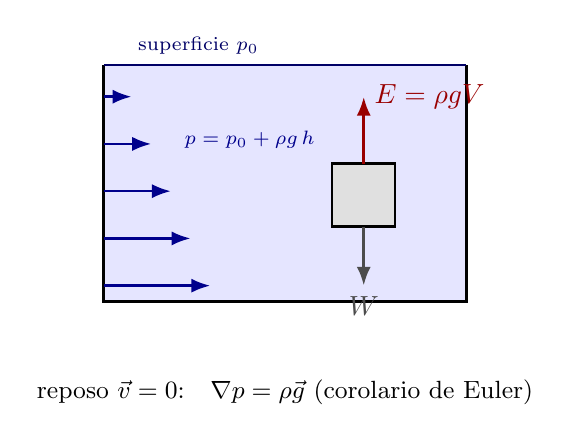
\begin{tikzpicture}[line width=0.9pt,>={Latex[length=2.4mm]}]
  \fill[blue!10] (0,0) rectangle (4.6,3);
  \draw[line width=1.1pt] (0,3)--(0,0)--(4.6,0)--(4.6,3);
  \draw[blue!40!black] (0,3)--(4.6,3); \node[blue!40!black] at (1.2,3.25){\scriptsize superficie $p_0$};
  \foreach \y/\l in {2.6/0.35,2.0/0.6,1.4/0.85,0.8/1.1,0.2/1.35}
     \draw[->,blue!55!black] (0,\y)--++(\l,0);
  \node[blue!55!black] at (1.85,2.05){\scriptsize $p=p_0+\rho g\,h$};
  % cuerpo sumergido
  \draw[fill=black!12] (2.9,0.95) rectangle (3.7,1.75);
  \draw[->,red!60!black,line width=1.2pt] (3.3,1.75)--++(0,0.85) node[right]{$E=\rho g V$};
  \draw[->,black!70,line width=1.1pt] (3.3,0.95)--++(0,-0.75) node[below]{$W$};
  \node at (2.3,-1.15){\small reposo $\vec v=0$:\quad $\nabla p=\rho\vec g$ (corolario de Euler)};
\end{tikzpicture}
\end{document}
